\documentclass[a4paper,12pt]{article}
\usepackage{graphicx}
\usepackage{bm,amssymb}
\usepackage{mathrsfs}
\usepackage[unicode,colorlinks=true,filecolor=blue, menucolor=black, linkcolor=black, citecolor=black,pagebackref=white]{hyperref}
\usepackage[utf8]{inputenc}
\usepackage[russian]{babel}
\usepackage{amsmath}
\usepackage{feynmp}
\usepackage{caption}
\usepackage{multicol}
\usepackage[inline]{enumitem}
\usepackage[left=2cm,right=2cm, top=2cm,bottom=2cm,bindingoffset=0cm]{geometry}
\begin{document}

\title{Семинар по теме: <<Интегралы с малым параметром>>}

\maketitle
На этом и следующих трёх занятиях будут рассмотрены интегралы, зависящие от параметра. При наличии малого параметра существует несколько способов оценить интеграл:
\begin{itemize}
	\item Разложение в ряд
	\item Выделение существенной области интегрирования
	\item Метод перевала или стационарной фазы
\end{itemize}
На данном семинаре будут рассмотрены первые 2 метода.
\section*{Ликбез}
Следующие интегралы будут часто использоваться в курсе:
\begin{equation}\label{eq:e1}
\int_{-\infty}^{+\infty} e^{-x^2} dx= \sqrt{\pi}
\end{equation}

\begin{equation}\label{eq:e2}
\int_{-\infty}^{+\infty} \frac{\sin x}{x}=\pi
\end{equation}

Вычислим первый (гауссов) интеграл:
$$
\left(\int_{-\infty}^{+\infty} e^{-x^2} dx\right)^2=\int_{-\infty}^{+\infty} dt \int_{-\infty}^{+\infty} dx e^{-x^2-t^2}=\int_{0}^{+\infty} r dr \int_{0}^{2\pi} d\varphi e^{-r^2}=\pi
$$
Извлекая корень, получаем ($\ref{eq:e1}$). Для вычисления ($\ref{eq:e2}$) рассмотрим интеграл:
$$
I(\lambda)=\int_{0}^{+\infty}\frac{\sin x}{x}e^{-\lambda x} dx
$$
На первый взгляд, этот интеграл сложнее исходного. Однако, при помощи дифференцирования по параметру $\lambda$, его можно существенно упростить, вычислить, а потом проинтегрировать обратно. Действительно, получаем:
$$
I^{'}(\lambda)=-\int_{0}^{+\infty}e^{-\lambda x}\sin x dx=Im\int_{0}^{+\infty}e^{-\lambda x+ix}=-Im\frac{1}{\lambda-i}=-\frac{1}{\lambda^2+1}
$$
Интегрируя, находим:
$$
I(\lambda)=-\arctan\lambda+C
$$
Константу найдём из рассмотрения предела $\lambda\to+\infty$. Имеем:
$$
I(\lambda)\approx0=C-\frac{\pi}{2}
$$
Отсюда, $C=\pi/2$ и $I(0)=\pi/2$.
Это был пример вычисления интеграла с параметром. Более подробно эта тема будет изучаться в лекции №3.

\subsection*{Оценка рядов}
В некоторых случаях можно с хорошей точностью оценить ряд при помощи формулы:
$$
\sum_{n=0}^{\infty} f(n)\approx\int_{0}^{\infty} dn f(n)
$$
Эта формула работает в случае
$$
\frac{|f(n)-f(n-1)|}{|f(n)|}\ll1
$$
\section*{Задача 1}

Найдём асимптотики интеграла при $x\gg1$ и $x\ll1$:
\[
I(x)=\int_{0}^{x}\frac{1-\cos t}{t}dt
\]



\subsection*{Решение}

Подынтегральная функция аналитична в нуле, поэтому при $x\ll1$ можно
просто разложить $\cos t$ в ряд Тейлора; имеем:
\[
I\left(x\right)\approx\int_{0}^{x}\frac{t^{2}/2}{t}dt=\frac{1}{4}x^{2}
\]

\noindent
При $x\gg1$, для интеграла важна вся область интегрирования; это
связано с тем, что при $x\to\infty$ этот интеграл расходится. Для
выделения ведущей асимптотики можно воспользоваться трюком. Во-первых,
поведение функции в нуле аналитично, поэтому интеграл можно представить
в виде:
\[
I\left(x\right)=\int_{0}^{1}\frac{1-\cos t}{t}dt+\int_{1}^{x}\frac{1-\cos t}{t}dt
\]
Поскольку на области интегрирования $\cos x$ успевает осциллировать
много раз, во втором слагаемом мы можем его выбросить (известно, что
$\int_{0}^{\infty}\frac{\sin x}{x}dx$ сходится и равен $\frac{\pi}{2}$,
поэтому при выбрасывании косинуса мы потеряем некую константу$\sim1$).
Во-вторых, поскольку подынтегральная функция аналитична в нуле, то
первое слагаемое тоже даст число $\sim1$. Таким образом формально
можно записать:
\[
I\left(x\right)=\int_{1}^{x}\frac{dt}{t}+O(1)\approx\ln x
\]

\noindent
На фоне большого слагаемого $\ln x\gg1$ (при $x\gg1$), выброшенные
константы порядка единицы являются малой добавкой. Это называется
взятием интеграла с логарифмической точностью. Точное вычисление асимптотики
дает ответ $\ln x+C+o(1)$, где $C\approx0.577$ - постоянная Эйлера-Маскерони.


\section*{Задача 2}

Найдём асимптотики интеграла при $a\gg b$ и $a\ll b$:
\[
I(a,b)=\int_{0}^{\infty}\frac{\exp(-x/a)}{\sqrt{x(x+b)}}dx
\]



\subsection*{Решение}

Обезразмерим интеграл, введя переменную $t=\frac{x}{a}$:
\[
I(a,b)\equiv I\left(\frac{b}{a}\right)=\int_{0}^{\infty}\frac{e^{-t}}{\sqrt{t\left(t+\frac{b}{a}\right)}}dt
\]



\paragraph{Случай $b\gg a$}

Из-за экспоненты, подыинтегральное выражение быстро затухает на масштабах
$t\sim1$ вблизи нуля. Поэтому в существенной области интегрирования
$t\ll\frac{b}{a}$ и в знаменателе можно выбросить $t$ на фоне большого
члена $\frac{b}{a}$. Имеем:

\[
I\left(\frac{b}{a}\right)\approx\sqrt{\frac{a}{b}}\int_{0}^{\infty}\frac{e^{-t}}{\sqrt{t}}dt = \sqrt{\frac{\pi a}{b}}
\]

\noindent
Заменой $t=z^{2}$ мы свели интеграл к известному интегралу Пуассона.



\paragraph{Случай $b\ll a$}

Тут экспонента тоже затухает очень быстро на масштабах $\sim1$. Однако,
если выбросить $\frac{b}{a}$ в знаменателе, мы получим расходящийся
интеграл - около нуля экспонента ведет себя примерно как $1$, и подынтегральная
функция имеет асимптотику $\sim\int_{0}^{\dots}\frac{1}{t}dt$,
то есть расходится логарифмически. Поэтому тут существенная область
интегрирования теперь - вблизи нуля. Интеграл можно переписать как:

\[
I\left(\frac{b}{a}\right)=\int_{0}^{1}\frac{e^{-t}}{\sqrt{t\left(t+\frac{b}{a}\right)}}dt+\int_{1}^{\infty}\dots
\]

\noindent
Второе слагаемое - сходящийся интеграл, который из-за экспоненты -
число порядка $1$ (формально можно оценить как $I_{2}<\int_{1}^{\infty}e^{-t}dt=\frac{1}{e}\sim1$);
на фоне большого первого слагаемого его можно выбросить. Далее, поскольку,
как было уже сказано, существенная область интегрирования лежит около
нуля, экспоненту можно положить равной $1$. Имеем:

\[
I\left(\frac{b}{a}\right)\approx\int_{0}^{1}\frac{1}{\sqrt{t\left(t+\frac{b}{a}\right)}}dt
\]

\noindent
Этот интеграл уже можно просто взять. Введем замену $t=z^{2}$:
\[
I\left(\frac{b}{a}\right)\approx\int_{0}^{1}\frac{2zdz}{\sqrt{z^{2}\left(z^{2}+\frac{b}{a}\right)}}=2\int_{0}^{1}\frac{dz}{\sqrt{z^{2}+\frac{b}{a}}}
\]

\noindent
Теперь введем замену $z=\sqrt{\frac{b}{a}}\sinh u$; тогда $z^{2}+\frac{b}{a}=\frac{b}{a}\left(\sinh^{2}u+1\right)=\frac{b}{a}\cosh^{2}u$:
\[
I\left(\frac{b}{a}\right)\approx2\int_{0}^{{\rm arcsinh}\sqrt{\frac{a}{b}}}\frac{\sqrt{\frac{b}{a}}\cosh udu}{\sqrt{\frac{b}{a}}\cosh u}=2{\rm arcsinh}\sqrt{\frac{a}{b}}
\]

\noindent
Для гиперболического арксинуса есть известное выражение через элементарные функции ${\rm arcsinh}x = \ln(a + \sqrt{a^2+1})$. Значит:
\[
I\left(\frac{b}{a}\right)\approx2\ln\left(\sqrt{\frac{a}{b}}+\sqrt{\frac{a}{b}+1}\right)\approx\ln\frac{a}{b}\gg1
\]

\noindent
(тут мы выбросили малые константные члены на фоне большой основной логарифмической асимптотики).


\section*{Задача 3}

Найдём асимптотики интеграла при $a\ll b$ и $a\gg b$:
\[
I\left(a,b\right)=\int_{0}^{\infty}\frac{\sin(\frac{x}{a})}{x(x^{2}+b^{2})}dx
\]



\subsection*{Решение}

Обезразмерим интеграл, введя переменную $t=\frac{x}{a}$:
\[
I\left(a,b\right)=\int_{0}^{\infty}\frac{\sin t}{at(a^{2}t^{2}+b^{2})}adt=\frac{1}{a^{2}}\int_{0}^{\infty}\frac{\sin t}{t\left(t^{2}+\frac{b^{2}}{a^{2}}\right)}dt\equiv\frac{1}{a^{2}}I\left(\frac{b}{a}\right)
\]



\paragraph{Случай $a\gg b$}

Если выбросить $\frac{b^{2}}{a^{2}}\ll1$ по сравнению с $t$ в знаменателе,
то мы получим расходящийся интеграл (в нуле как $\sim\int_{0}^{\dots}\frac{dt}{t^{2}}$).
Из этого можно заключить, что основная область, где интеграл набирается
- вблизи нуля. Поэтому $\sin t$ можно разложить; имеем:
\[
I\left(\frac{b}{a}\right)\approx\int_{0}^{\infty}\frac{dt}{t^{2}+\left(\frac{b}{a}\right)^{2}}=\frac{a}{b}\left.\arctan\left(\frac{b}{a}t\right)\right|_{0}^{\infty}=\frac{\pi a}{2b}\Rightarrow I(a,b) = \frac{\pi}{2 a b}
\]

\paragraph{Случай $a\ll b$}

Поскольку интеграл от функции $\frac{\sin t}{t}$ набирается на масштабах
порядка $\sim1$ (из-за осциллирующего синуса), то в знаменателе можно
выбросить $t^{2}$ на фоне $\frac{b^{2}}{a^{2}}\gg1$. Имеем:
\[
I\left(\frac{b}{a}\right)\approx\int_{0}^{\infty}\frac{\sin x}{x\frac{b^{2}}{a^{2}}}dx=\frac{\pi}{2}\cdot\frac{a^{2}}{b^{2}} \Rightarrow I(a,b) \approx \frac{\pi}{2 b^2}
\]

\section*{Задача 4}

Вычислить в главном приближении интеграл:

$$
I=\int_{0}^{2\pi}d\theta \exp\left[-\alpha\left(\frac{\theta}{2}+\sin\theta\right)\right],
$$
а также найти первую ненулевую поправку к нему в двух случаях:
\begin{multicols}{2}
\begin{enumerate}[label=\arabic*)]
    \item $\alpha\ll1$;
    \item $\alpha\gg1$.
\end{enumerate}
\end{multicols}
\noindent

\subsection*{Решение}

\paragraph{Случай $\alpha\ll 1$}

На всей области интегрирования аргумент экспоненты мал и можно пользоваться разложением в ряд Тейлора:

\[
I\approx\int_{0}^{2\pi}d\theta\left(1-\alpha\left(\frac{\theta}{2}+\sin\theta\right)\right)=2\pi\left(1-3\pi\alpha/2\right).
\]

\paragraph{Случай $\alpha\gg 1$}

В этом случае интеграл набирается вблизи 0 (см. рис.).

\begin{figure}[ht]
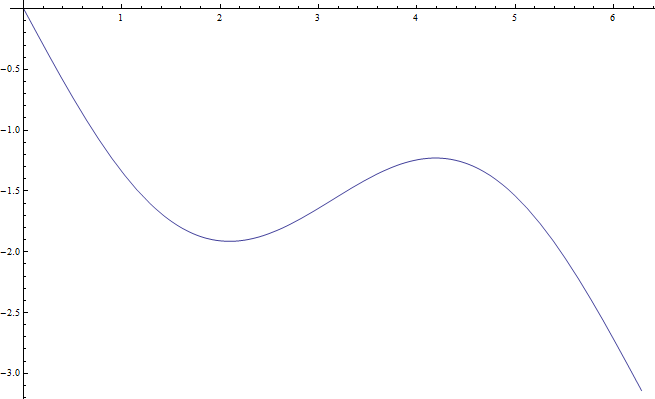
\includegraphics[width=0.8\linewidth]{Task_4.png}
\caption{График функции $\frac{\theta}{2}+\sin\theta$.}
\label{exp_plot}
\end{figure}

\noindent
В первом приближении получаем:

\[
I\approx\int_0^{2\pi}d\theta\exp\left[-\frac{3}{2}\alpha\theta\right]=\frac{2}{3\alpha}\left(1-e^{-3\pi\alpha}\right)\approx\frac{2}{3\alpha}.
\]
Заметим, что в данном случае $e^{-3\pi\alpha}$ не является первой поправкой. Действительно, дополнительным источником поправок является разложение синуса в экспоненте до кубического члена и далее. Т.к. интеграл набирается на $\theta\sim\alpha^{-1}$, то поправка от разложения синуса будет иметь степенную малость ($\sim\alpha^{-3}$), а не экспоненциальную. Найдём теперь численный коэффициент перед этой поправкой:

\[
I\approx\int_0^{2\pi}d\theta\exp\left[-\frac{3}{2}\alpha\theta+\alpha\theta^3/6\right]\approx\frac{2}{3\alpha}+\frac{1}{6}\alpha\int_0^{2\pi}d\theta\theta^3e^{-3\alpha\theta/2}\approx\frac{2}{3\alpha}+\frac{16}{81\alpha^3}.
\]
В последнем равенстве мы опять отбросили граничные члены в интеграле из-за их экспоненциальной малости.

\newpage

\section*{Задачи для домашнего решения}
\noindent \textbf{Упражнение 1}

\noindent Пусть $a,b>0$. Найдите асимптотическое выражение для следующего интеграла:
\begin{equation}\notag
I(a,b)=\int_{0}^{\infty}e^{-ax}\frac{\sin^{2}bx}{x^{2}}dx	
\end{equation}
\noindent при а) $a\gg b$ и б) $a\ll b$ (здесь и далее можно ограничиться главным порядком малости и все параметры считать положительными).

\vspace{15pt}
\noindent \textbf{Упражнение 2}

\noindent Найдите асимптотическое выражение для следующего интеграла:
\begin{equation}\notag
\int_{0}^{\infty}\frac{1}{x^{2}+a^{2}}\frac{1}{(x-1)^{2}+b^{2}}dx
\end{equation}
\noindent при а) $a\ll 1$,\quad $b\sim 1$ и б) $a=b\gg1$.

\vspace{15pt}
\noindent \textbf{Упражнение 3}

\noindent Найдите асимптотическое выражение для следующего интеграла:
\begin{equation}\notag
I(a,b)	=\int_{0}^{\infty}\frac{x}{x^{2}+a^{2}}(1-\tanh bx)dx
\end{equation}
\noindent При $b\ll 1$ и $a\ll 1$.

\vspace{15pt}
\noindent \textbf{Упражнение 4}

\noindent Приближенно вычислите сумму
\begin{equation}\notag
S(a,b)	=\sum_{n=0}^{\infty}n^{a}e^{-bn}
\end{equation}

\noindent при а) $a\sim 1$ и $b\ll 1$, б) $b\gg\frac{a}{b}\gg 1$. Параметр $a$ считать натуральным числом.

\vspace{15pt}
\noindent \textbf{Задача 1}

\noindent Найдите асимптотическое выражение для следующего иниеграла:
\begin{equation}
\notag
I(a)=\int_{0}^{\infty}\frac{1}{xa^{2}+(1-x^{2})^{2}}dx	
\end{equation}

\noindent при a) $1\gg a$, б) $1\ll a$.

\vspace{15pt}
\noindent \textbf{Задача 2}

\noindent Найдите асимптотическое выражение для следующего интеграла:
\begin{equation}\notag
I(n,a,b)	=\int_{0}^{a}\frac{x^{n}}{e^{x/b}-1}dx
\end{equation}
\noindent при а) $b\gg a$ и б) $n\gg 1$, $nb\ll a$. Параметр $n$ предполагается натуральным числом.

\end{document}
